\documentclass[9pt,twoside,lineno]{pnas-new}
% Use the lineno option to display guide line numbers if required.

\templatetype{pnassupportinginfo}

\title{Local similarity and global variability characterize the semantic space of human languages}

% Use letters for affiliations, numbers to show equal authorship (if applicable) and to indicate the corresponding author
\author{Lewis, M., Cahill, A., Madnani, N., Evans, J.}

\correspondingauthor{Corresponding authors: Molly Lewis (mollylewis@cmu.edu) or James Evans (jevans@uchicago.edu)}

\begin{document}

%% Comment out or remove this line before generating final copy for submission; this will also remove the warning re: "Consecutive odd pages found".
%\instructionspage  

\maketitle

%% Adds the main heading for the SI text. Comment out this line if you do not have any supporting information text.
%\SItext



%\section*{Fig. S1}
\begin{figure}
\centering
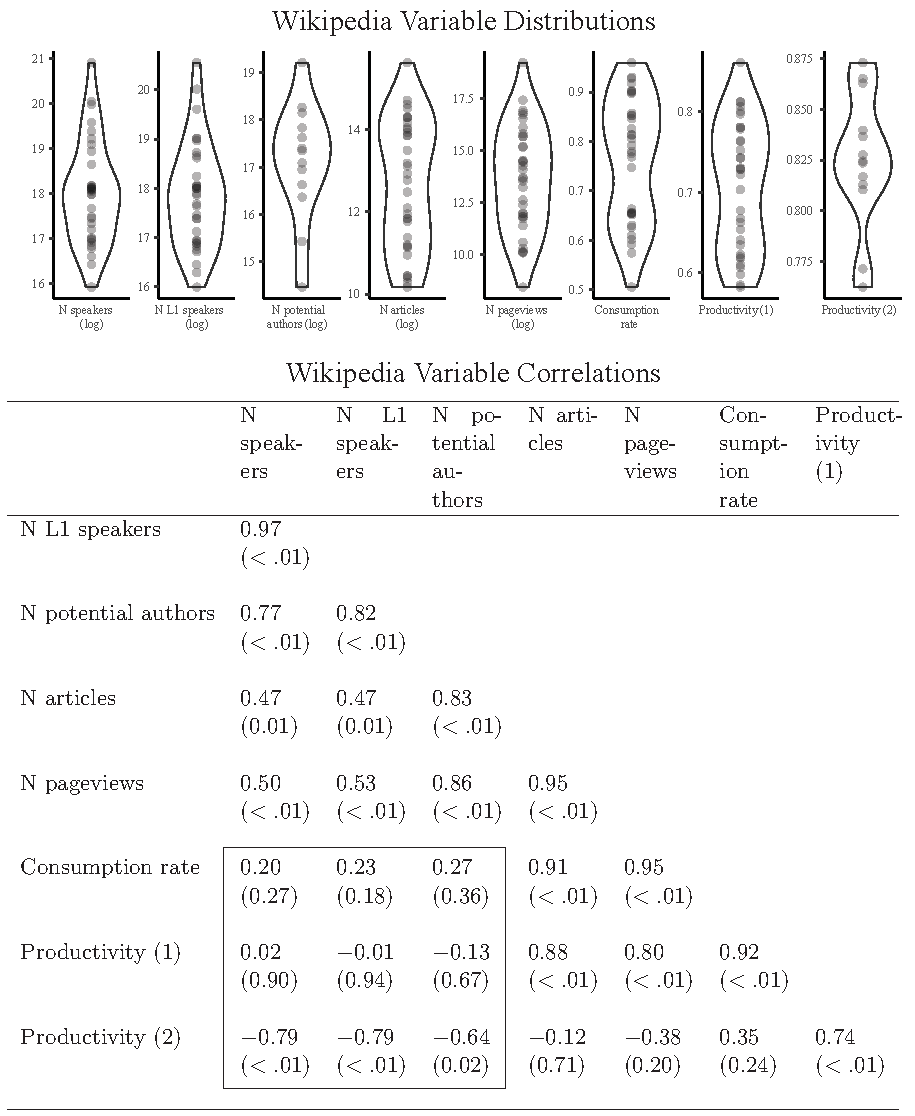
\includegraphics[width = 5.2in]{suppfigs/wiki_distribution_correlation.pdf}


%\pagebreak
%\clearpage
  \caption{{\it Top}: Distributions for eight descriptive statistics associated with multi-lingual Wikipedia corpora. N speakers indicates the log number of first and second language speakers (N languages missing = 1) \cite{wikispeakers}; N L1 speakers indicates the log number of first language speakers only (N missing = 1) \cite{amano2014global}. N potential authors estimates the log number speakers of the target language who have access to the internet, and have sufficient command of the target language to author an article (N  missing = 22) \cite{wikiproductivity}. N articles indicates the log number of articles by language (31 March 2015; N  missing = 1) \cite{wikispeakers}. N pageviews indicates the log number of pageviews by language for a 24 hour period (1 August 2016) \cite{wikipageview}. Consumption rate is the log number of articles / log number of first language speakers (N  missing = 1). Productivity (1) is the log number of articles / log number of first language speakers (N  missing = 2). Productivity (2) is the log number of articles / log number of potential authors (N  missing = 22). Each point corresponds to a language. {\it Bottom}: Pairwise correlations between Wikipedia measures (Pearson's $r$). Parenthetical numbers indicate p-values. Critically, languages with more speakers do not have greater rates of engagement, as measured by number of articles written and viewed relative to the number of speakers. In fact, by one measure of article production (Productivity (2)), languages with more speakers write relatively fewer articles per speaker capita.}
\end{figure}

\pagebreak
\clearpage


%\section*{Fig. S2}

\begin{figure}[h]
\centering
\includegraphics[width=16.7cm]{suppfigs/distinctiveness_fig.pdf}


  \caption{Essays written in English by speakers of the same native language are more semantically similar than essays written by speakers of different native languages, corroborating informal observations by second language educators and bilingual researchers in individual pairs of languages second language speakers appear to ``think'' in their first language \cite{wu2014influence, filipovic2018speaking}. We evaluated language semantic distinctiveness by analyzing the position of essays in semantic space for a model trained on all essays in all languages. For each language, we averaged the cosine distance between essay pairs from the same language (``within"), and averaged  pairs between different languages (``between").  We then quantified language-level semantic distinctiveness in two ways: (1) the difference between the two measure (within - between) as in \cite{kozlowski2019geometry, bodell2019interpretable, an2018semaxis, kwak2020frameaxis}, and (2) the ratio between them (within/between) as in \cite{levy2014linguistic, levy2014neural, levy2015improving}. Both types of measures have been shown to capture meaningful semantic relationships in embedding models. In the Main Text, we report the results for the difference measure; here we replicate our results with the ratio measure. The ratio is greater than one when languages are located in a distinct semantic space, relative to other languages. This value was substantially greater than one for all languages in our sample ($M$ = 1.26; $SD$ = .09; $t$(34) = 17.09; $p$ $<$ .00001). We also conducted  this analysis for two types of essays separately: low scoring essays (score $<$ 4 on 5 pt.\ scale) and high scoring essays (score $\geq$ 4).  Low scoring essays ($M$ = 1.27; $SD$ = .08) were more distinct than high scoring essays ($M$ = 1.21; $SD$ = .09; $t$(34) = 5.73; $p$ $<$ .00001).  Main panel shows mean distinctiveness value across samples with the ratio measure.  Red bars correspond to high scoring essays; blue bars correspond to low scoring essays. Ranges indicate bootstrapped 95\% confidence intervals. Upper right panel shows the distribution of essay scores (1-5) for the 38,500 essays in the TOEFL corpus ($M$ = 3.51; $SD$ = .91).}
\end{figure}

\pagebreak
\clearpage


%\section*{Fig. S3}
\begin{figure}[h]
\centering
     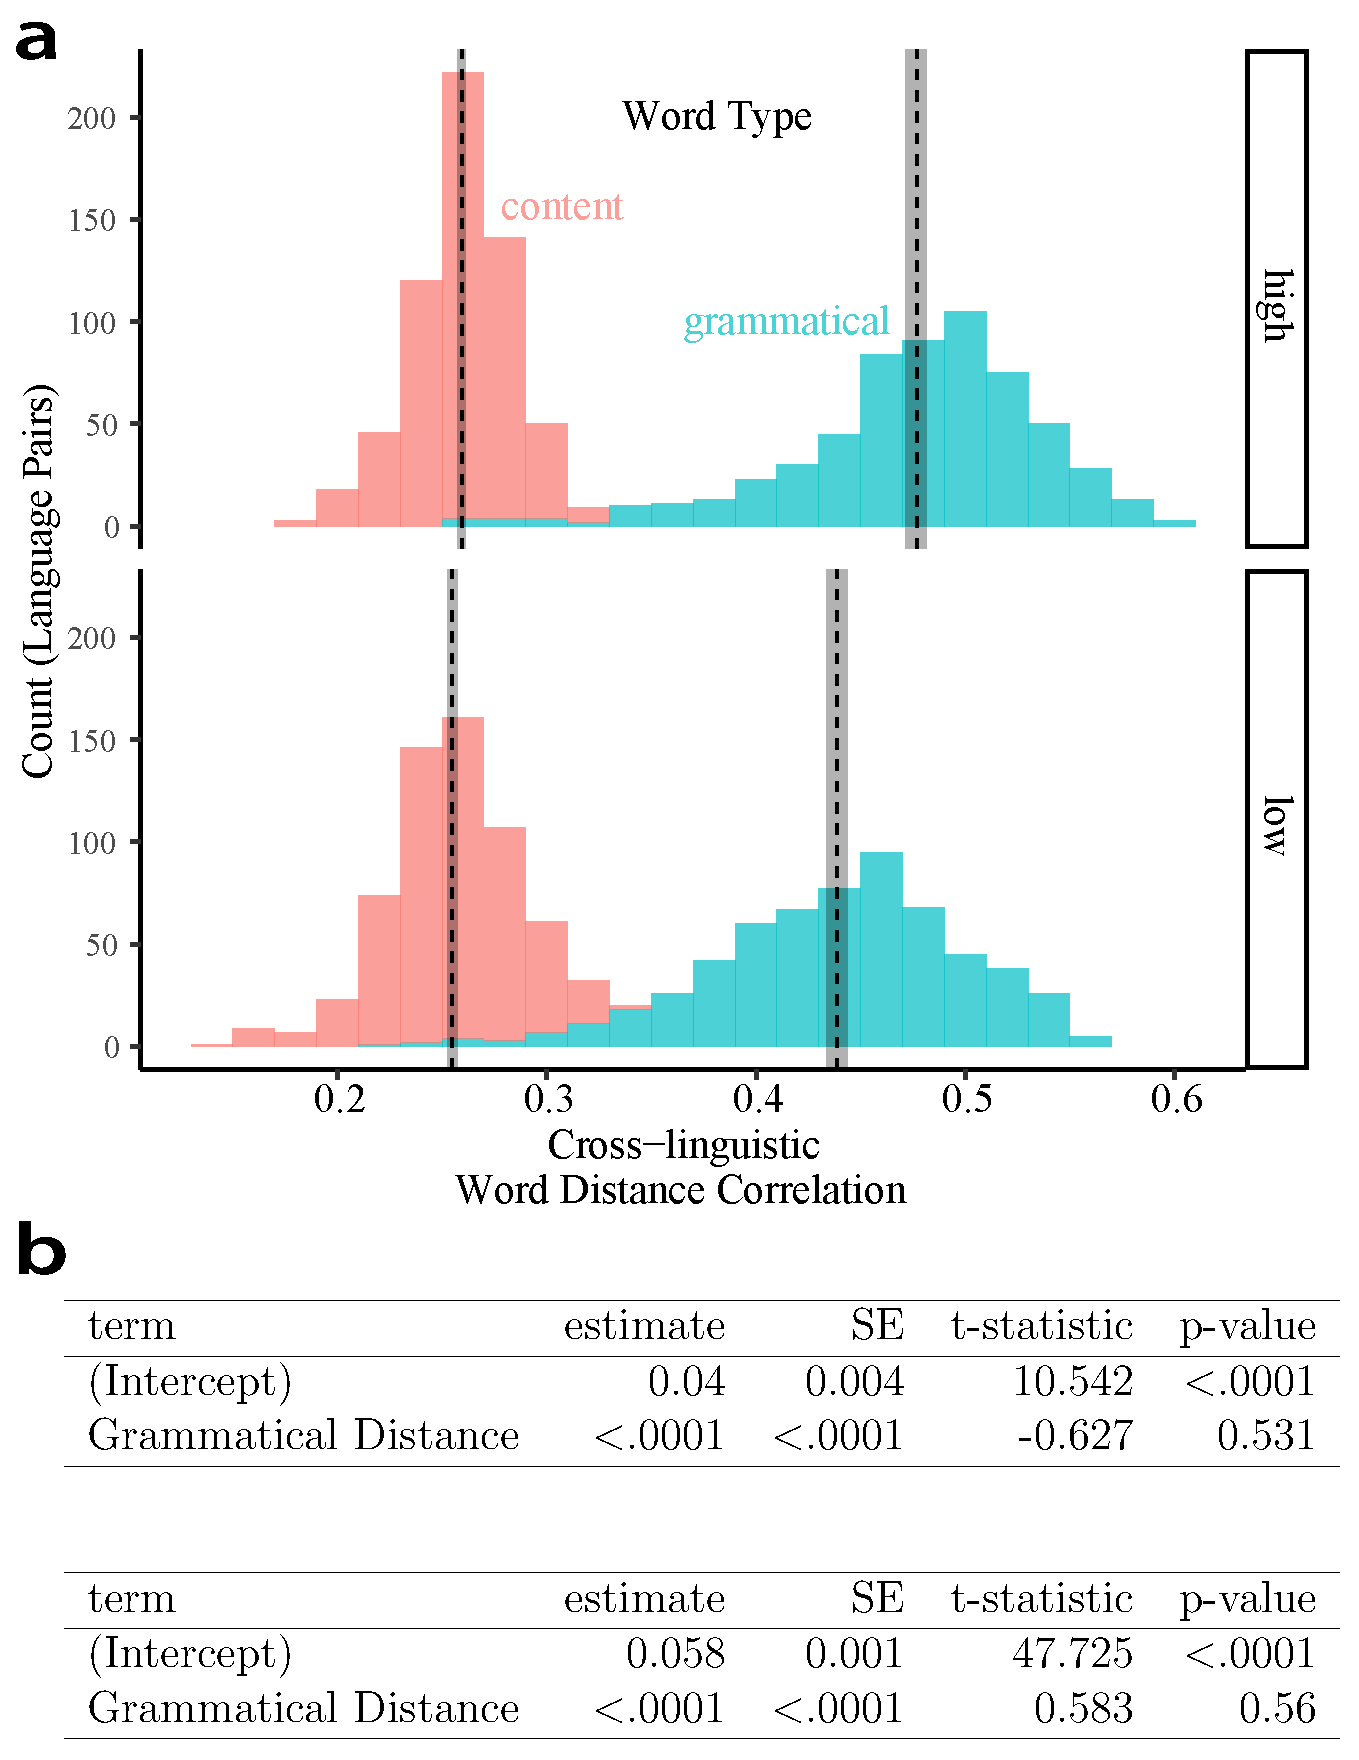
\includegraphics[width=4.5in]{suppfigs/syntax_control.pdf}

  \caption{{\textbf a.} Grammatical words (e.g., ``and", ``the") are more similar across languages than content words (e.g., ``love"). In Jakobson's functional typology \cite{jakobson1990language}, grammatical words are \textit{metalingual}--they govern the structure of the code of language itself and so play a related function across languages. As such, grammatical words are qualitatively different from abstract content words such as ``career" or ``government" that vary based on distinctive complex cultural environments. We divided the words from the TOEFL essays analyzed in the Main Text ($N$ = 3,530) into two sets -- ``content" and ``grammatical"  -- based on  part of speech information from \cite{brysbaert2012adding}. Nouns, verbs, adverbs, adjectives, or interjections were categorized as content ($N$ = 3,339); articles, determiners, conjunctions, pronouns, or prepositions ($N$ = 145) were categorized as grammatical. We then calculated the cosine distance between each word pair within a word type (content or grammatical) for models trained separately on low and high scoring essays for essays written by speakers of each of 35 different native languages. Finally, we compared the distances between words across language pairs (e.g., correlation of distances for content words based on essays written by native Spanish versus native French speakers). {\it x}-axis shows magnitude of cross-linguistic word distance correlation (Pearson's $r$); {\it y}-axis shows counts of language pairs. Facets show results from models trained on low (score $<$ 4 on 5 pt.\ scale; bottom) and high (score $\geq$ 4; top) scoring essays. Color indicates word type. Vertical lines indicate distribution means with bootstrapped 95\% confidence intervals. {\textbf b.} Model results predicting the difference between local and global word correlations by language pair ($N$ = 595). Intercept parameter  compares local-global difference to zero; Grammatical distance predictor measures typological distance between languages based on the WALS database \cite{dediu2018trees,wals2013}. Top table shows results for Wikipedia corpus; Bottom table shows results for TOEFL corpus. These models suggest that languages are more similar locally, relative to globally, and that this difference is not predicted by grammatical similarity between languages.}
  \end{figure}

\pagebreak
\clearpage


%\section*{Fig. S4}
\begin{figure}[h]
\centering
\includegraphics[width=5in]{suppfigs/concreteness_plot_random.pdf}

 \caption{An alternative explanation for the finding that concrete words are more similar cross-linguistically  relative to abstract words is that concrete words, in general, tend to appear in more similar contexts in corpora of text relative to abstract words. To test this possibility, we constructed 35 corpora with each corpus containing equally-sized samples of TOEFL essays  from each of the 35 different languages. Each corpus was therefore comparably sized to the language-based corpora described in the Main Text (approx.\ 1100 essays), but contained essays written by speakers of all 35 native languages. We then calculated mean pairwise correlation between word distances across languages as a function of the concreteness decile of the words. Point ranges correspond to bootstrapped 95\% confidence intervals; range on model fit corresponds to the standard error. Unlike for the language-based corpus, there is no effect of concreteness on cross-corpus similarity: Across corpora, low and high concrete meanings are equally similar ($r$ = .02; $p$ = .96). This suggests that the concreteness effect reported in the Main Text is due to cross-linguistic differences in meanings, rather than an artifact of, e.g., differing types of linguistic contexts for high versus low concrete words. }

\end{figure}


\pagebreak
\clearpage


%\section*{Fig. S5}

\begin{figure}[h]
\centering
\includegraphics[width=5in]{suppfigs/conc_freq_control.pdf}
\caption{ Mean word frequency for words in each concreteness decile from the TOEFL corpus. Word frequency is estimated from the actual word counts in the corpus. Error bars are bootstrapped 95\% confidence intervals. This analysis suggests that more concrete words tend to be less frequent in the corpus, making it unlikely that the relationship between concreteness and cross-linguistic similarity is due to measurement noise.}
\end{figure}

\pagebreak
\clearpage


%\section*{Fig. S6}

\begin{figure}[h]
\centering
     \includegraphics[width=6in]{suppfigs/swadesh_plot_ED.pdf}
 \caption{Physical distance between two languages predicts semantic similarity of Swadesh meanings between two languages: Languages that are geographically closer have more similar meanings. Each facet corresponds to a Swadesh word. Each point shows the correlation between the pairwise distances between the target Swadesh word and all other Swadesh words for a language pair (e.g., a point on the ``earth" facet represents the magnitude of the correlation between Spanish and French of  the distances between ``earth" and all other Swadesh words). Physical distance  in meters (millions) between languages is plotted on the x-axis and magnitude of correlation between distances to other Swadesh items is plotted on the y-axis. All correlations are significant at the $\alpha$ = .01 level except the items ``star" (QAP $p$ = .016) and ``lake" (QAP $p$ = .119).}
 \end{figure}


\pagebreak
\clearpage




%\section*{Fig. S7}

\begin{figure}[h]
\centering
     \includegraphics[width=4.5in]{suppfigs/distance_regressions.pdf}


 \caption{{\textbf a.} Language pairwise predictors of semantic similarity for full sample of 35 languages. Cultural language distances were not available for 7 of the 35 languages in our sample (German, Greek, Italian, Portuguese, Romanian, Farsi, and Yoruba). In the Main Text, we report model parameters for the set of 28 languages for which we have full data. Here, we show model parameters for the other predictors for the full sample of 35 languages.  Red points indicate standardized estimates from a single-predictor model; grey points indicate estimates from additive linear model with all five predictors included. Ranges are 95\% confidence intervals. {\textbf b.} Cultural predictors of semantic distance for each of 10 cultural sub-domains.  Points are standardized estimates from an additive linear model with all five predictors included. Ranges are 95\% confidence intervals.}
 
 \end{figure}


\pagebreak

\clearpage

%\section*{Fig. S8}

\begin{figure}[h]
\centering
\includegraphics[width = 6.3in]{suppfigs/continuous_semantic_clusters.pdf}
   \caption{As described in the Main Text, we clustered the words  into 10 clusters for each of the two corpora (Second-Language TOEFL and Multilingual Wikipedia). Each point in the figure corresponds to a unique pair of clusters. The y-axis shows the average correlation (Pearson's {\it r}) in pairwise word distances between the two clusters across all language pairs (e.g., correlation of all word pair distances between the 1-2 cluster pair for French and Spanish, and all other language pairs). The x-axis shows the cosine distance between the centroids of the two clusters. Color indicates whether the two clusters are the same  (``local;" red) or different (``global;" blue). There is a positive correlation between cluster centroid distance and the magnitude of the pairwise word correlation for both corpora (TOEFL: $r$ = .39, $p$ = .003; Wikipedia: $r$ = .34, $p$ = .01). Notably, however, there is a bimodal relationship in centroid distances characterized by the local-global distinction.}
\end{figure}


\pagebreak
\clearpage


% latex table generated in R 3.6.1 by xtable 1.8-4 package
% Mon May 25 13:36:50 2020
%\begin{sidewaystable}



%\section*{Fig. S9}

\begin{figure}[h]
\centering
     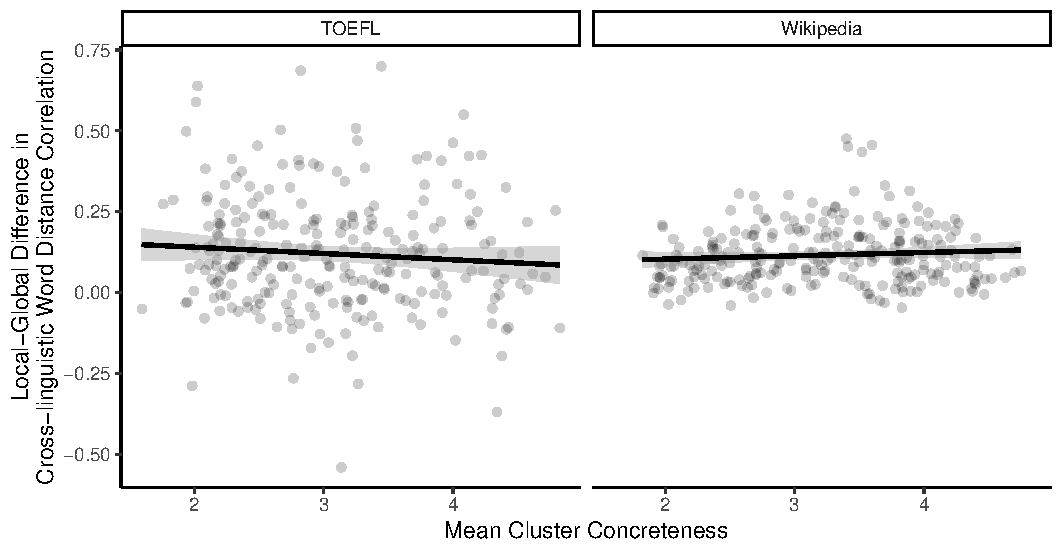
\includegraphics[width = 6.3in]{suppfigs/local_global_concreteness_semantics_plot.pdf}
         \caption{Relationship between cluster concreteness and the magnitude of the local-global effect for the 250 cluster solution for TOEFL (left) and Wikipedia (right). For each cluster in each corpus, we calculated the mean concreteness of words in that cluster and the mean cross-linguistic correlation in word pairwise distances within the same cluster (local) versus across different clusters (global). The {\it y}-axis shows the difference in local versus global correlations  aggregating across language pairs. Larger values indicate that word meanings are more similar within clusters versus across. Each point corresponds to a cluster. These results reveal that, while semantic clusters tend to co-vary with concreteness, the concreteness of a cluster is not predictive of the local-global effect. }
\end{figure}

\pagebreak
 \clearpage
 
 %\section*{Fig. S10}
 
\begin{figure}[h]
\centering
     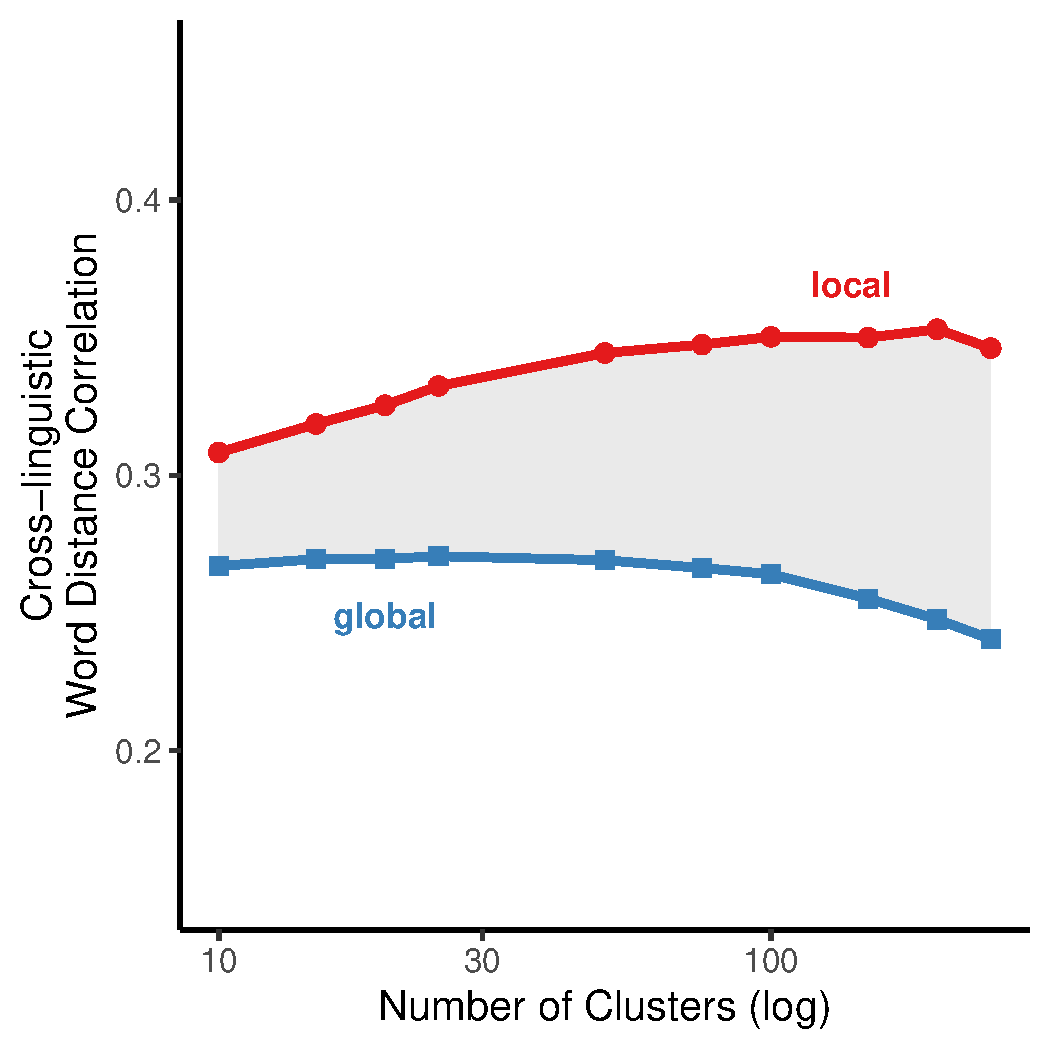
\includegraphics[width = 5in]{suppfigs/native_clustering_local_global}
         \caption{Cross-linguistic word distance correlations for local (red) versus global (blue) semantic comparison as a function of the number of semantic clusters using native model clusters for models trained on TOEFL essays. In Fig. 3D of the Main Text, we demonstrate that distances within clusters (local) are more correlated with each other cross-linguistically than word distances across clusters (global). This analysis was based on clusters defined by a model trained on English Wikipedia articles. Here, we replicate this pattern using clusters determined by models trained on native language text. For example, when comparing TOEFL essays from native Hindi and Mandarin speakers, we clustered words covering the Hindi and Chinese Wikipedia entries to capture how each language represents its knowledge base. Then we compared within Hindi-Wikipedia-clusters vs. between Hindi-Wikipedia-clusters for essays from native speakers of both languages; next we compared within Mandarin-Wikipedia-clusters vs. between Mandarin-Wikipedia clusters for the same essays; finally we averaged these differences. }
\end{figure}

\pagebreak
 \clearpage

%\section*{Fig. S1}

\begin{table}[h]
\centering
\begin{tabular}{llp{1.5cm}p{1.8cm}p{1.3cm}p{1.3cm}p{1.3cm}p{1.3cm}}

  & &  Semantic   &  Grammat-ical   &  Physical   &  Climate  &  Lexical    &  Cultural  \\ 
  \hline
    \hline
{\it 35 languages} & Semantic  & 1.00 & & &  & \\ 
& Grammatical  & 0.55 & 1.00 &  & & \\ 
& Physical  & 0.52 & 0.46 & 1.00 &  & \\ 
& Climate  & 0.55 & 0.35 & 0.55 & 1.00 & \\ 
& Lexical  & 0.71 & 0.60 & 0.45 & 0.45 & 1.00 \\ 
   \hline
  % \hline
{\it 28 languages} &   Semantic  & 1.00 &  &  & &  & \\ 
 &Grammatical  & 0.61 & 1.00 &  &&  & \\ 
&Physical  & 0.52 & 0.53 & 1.00 & & &\\ 
& Climate  & 0.54 & 0.41 & 0.58 & 1.00  &  &\\ 
&  Lexical  & 0.73 & 0.63 & 0.47 & 0.49& 1.00 & \\
&    Cultural  & 0.69 & 0.47 & 0.49 & 0.59 & 0.72  & 1.00\\ 
      \hline
        \hline
\end{tabular}
   \caption{ {\it Top:} Pairwise correlations (Pearson's {\it r}) between language distances measures for all 35 languages (excluding cultural distance measure which has  missing data). {\it Bottom:} Pairwise correlations (Pearson's {\it r}) between language distance measures for the subset of 28 languages for which data is available for all 6 predictors. All correlations are significant at the $\alpha$ = .05 level using QAP tests.} 
\end{table}

\pagebreak
 \clearpage




% For your review copy (i.e., the file you initially send in for
% evaluation), you can use the {figure} environment and the
% \includegraphics command to stream your figures into the text, placing
% all figures at the end.  For the final, revised manuscript for
% acceptance and production, however, PostScript or other graphics
% should not be streamed into your compliled file.  Instead, set
% captions as simple paragraphs (with a \noindent tag), setting them
% off from the rest of the text with a \clearpage as shown  below, and
% submit figures as separate files according to the Art Department's
% instructions.


\bibliography{L2ETS_bib}

\end{document}
